% Build from the repository root with:
% latex -output-directory=figures figures/Figure2.tex
% dvips -o figures/Figure2.ps figures/Figure2.dvi
% ps2epsi figures/Figure2.ps figures/Figure2.eps
\documentclass{minimal}
\usepackage{tikz}
\usetikzlibrary{arrows.meta}

\newcommand{\Rpos}{\mathcal{P}}
\newcommand{\Rneg}{\mathcal{R}}
\newcommand{\Jord}{\mathcal{J}}
\newcommand{\orderfactor}{\mathcal{B}}

\begin{document}
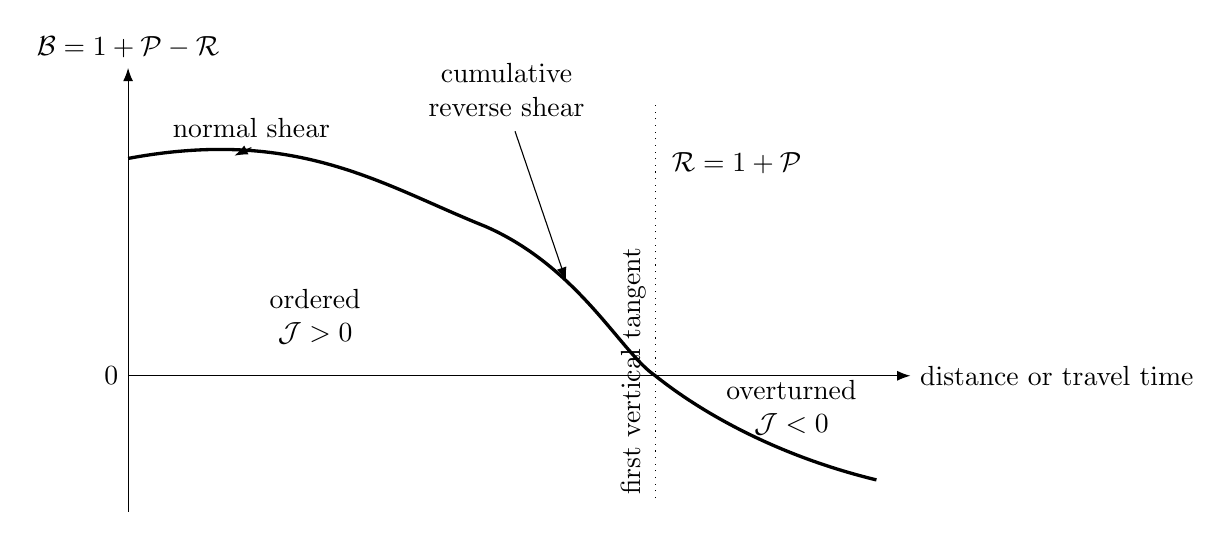
\begin{tikzpicture}[x=1.08cm,y=1.15cm,>=Latex]
  \draw[->] (0,0) -- (9.2,0) node[right] {distance or travel time};
  \draw[->] (0,-1.5) -- (0,3.4) node[above] {$\orderfactor=1+\Rpos-\Rneg$};
  \draw[dashed] (0,0.0) -- (9,0.0);
  \node[left] at (0,0) {$0$};
  \draw[very thick] (0,2.4) .. controls (2.0,2.75) and (3.0,2.1) .. (4.2,1.65)
    .. controls (5.3,1.2) and (5.8,0.25) .. (6.2,0)
    .. controls (6.8,-0.45) and (7.7,-0.9) .. (8.8,-1.15);
  \draw[dotted] (6.2,-1.35) -- (6.2,3.0);
  \node[right] at (6.28,2.35) {$\Rneg=1+\Rpos$};
  \node[align=center] at (2.2,0.65) {ordered\\$\Jord>0$};
  \node[align=center] at (7.8,-0.35) {overturned\\$\Jord<0$};
  \node[rotate=90,anchor=south] at (6.2,0.05) {first vertical tangent};
  \draw[->,thin] (1.45,2.52) -- (1.25,2.43);
  \node[above] at (1.45,2.52) {normal shear};
  \draw[->,thin] (4.55,2.70) -- (5.15,1.05);
  \node[above,align=center] at (4.45,2.76) {cumulative\\reverse shear};
\end{tikzpicture}
\end{document}
